\documentclass[12pt, a4paper]{report}

\usepackage[czech]{babel}
\usepackage[utf8]{inputenc}
%\usepackage[cp1250]{inputenc}
\usepackage[IL2]{fontenc}
\usepackage{anyfontsize}
\usepackage{graphicx}
\usepackage{float}
\usepackage{color}

\title{Manuál aplikace MediTab}
\author{David Pivovar}

%%%%%%%%%%%%%%%%%%%%%%%%%%%%%%%%%%%%%%%%%%%%%%%%%%%%%%%%%%%
%%%%%Makra%%%%%%%%%%%%%%%%%%%%%%%%%%%%%%%%%%%%%%%%%%%%%%%%%

% Tato makra přesvědčují mírně ošklivým trikem LaTeX, aby hlavičky kapitol
% sázel příčetněji a nevynechával nad nimi spoustu místa. Směle ignorujte.
\makeatletter
\def\@makechapterhead#1{
  {\parindent \z@ \raggedright \normalfont
   \Huge\bfseries \thechapter. #1
   \par\nobreak
   \vskip 20\p@
}}
\def\@makeschapterhead#1{
  {\parindent \z@ \raggedright \normalfont
   \Huge\bfseries #1
   \par\nobreak
   \vskip 20\p@
}}
\makeatother

% Toto makro definuje kapitolu, která není očíslovaná, ale je uvedena v obsahu.
\def\chapwithtoc#1{
\chapter*{#1}
\addcontentsline{toc}{chapter}{#1}
}



%%%%%%%%%%%%%%%%%%%%%%%%%%%%%%%%%%%%%%%%%%%%%%%%%%%%%%%%%%%
%%%%%Zacatek dokumentu%%%%%%%%%%%%%%%%%%%%%%%%%%%%%%%%%%%%%

\begin{document}

%%%%%%%%%%%%%%%%%%%%%%%%%%%%%%%%%%%%%%%%%%%%%%%%%%%%%%%%%%%
%%%%%Titulni strana%%%%%%%%%%%%%%%%%%%%%%%%%%%%%%%%%%%%%%%%
\begin{titlepage}

\begin{center}

\vspace*{50pt}
	
	{\fontsize{36}{0} \textbf{
		{\color{red}MediTab}
	}}
	
	\vfill
	
	{\fontsize{28}{0} \textbf{
		Manuál
	}}
	
	\vfill
	\vfill
	
	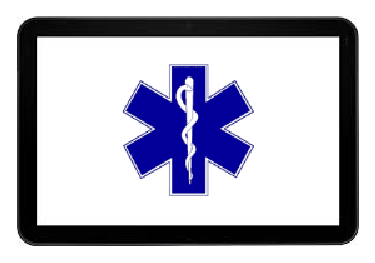
\includegraphics[width=0.7\textwidth]{img/logo_wide.eps}

\end{center}

\vspace{110pt}

\begin{flushleft}

	{\fontsize{20}{0} \selectfont
		David Pivovar\\[5pt]
		%Daniel Švarc
		\hfill
		Verze 1.0
	}
	
\end{flushleft}

\end{titlepage}


\tableofcontents

%%%%%%%%%%%%%%%%%%%%%%%%%%%%%%%%%%%%%%%%%%%%%%%%%%%%%%%%%%%
%%%%%Kapitoly%%%%%%%%%%%%%%%%%%%%%%%%%%%%%%%%%%%%%%%%%%%%%%

\setlength{\parskip}{1em}

\chapter*{Úvod}
\addcontentsline{toc}{chapter}{Úvod}
\chapter{Manuál}

%%%%%%%%%%%%%%%%%%%%%%%%%%%%%%%%%%%%%%%%%%%%%%%%%%%%%%%%%%%


\end{document}
